\documentclass[11pt]{article}
% \usepackage[french]{babel}
%  \usepackage{DejaVuSans}
%  \usepackage{libertine}
%  \renewcommand*\rmdefault{cmfib} 
% \usepackage[default]{cantarell}

% \usepackage[T1]{fontenc}
% \renewcommand{\rmdefault}{cmss}  
% \fontencoding{T1}
%   \fontfamily{cmss}
%   \fontseries{m}
%   \fontshape{n}
%   \fontsize{10}{15}
% \renewcommand*\familydefault{cmss}
%   \selectfont
% \usepackage[utf8]{inputenc} 
\usepackage{array, xcolor, lipsum, bibentry}
\usepackage[top=0.7cm, bottom=1.5cm, left=1.9cm, right=1.9cm]{geometry} 
% \usepackage[margin=2.0cm]{geometry} 
%lmargin=3.0cm, rmargin=1.0cm,tmargin=2.50cm,bmargin=2.50cm
\usepackage{longtable}
\usepackage{fancyheadings}
 \pagestyle{fancyplain}
 \fancyhead{}
\fancyfoot{}
\renewcommand{\headrulewidth}{0pt}
\cfoot{\thepage}
\rfoot{\scriptsize \selectfont Iliya Enchev \longdate{\today}}
% \usepackage{helvet}
% \usepackage[french]{babel}
% \usepackage[T1]{fontenc}
% \usepackage[utf8]{inputenc}

% \usepackage[T1]{fontenc}
\usepackage{graphicx}
\usepackage[light,math]{iwona} 
% \usepackage{DejaVuSans}
%   \renewcommand{\rmdefault}{cmss}  
%   \renewcommand{\sfdefault}{cmr}
%   \renewcommand{\ttdefault}{ptm}

%     \usepackage{titlesec}
%     \titleformat{\section}{\large\bfseries}{\thesection}{1em}{}

\newcommand{\addphoto}[2]{%
  \smash{%
    \makebox[0pt][l]{%
      \raisebox{#1pt}{%
        \hspace{#2pt}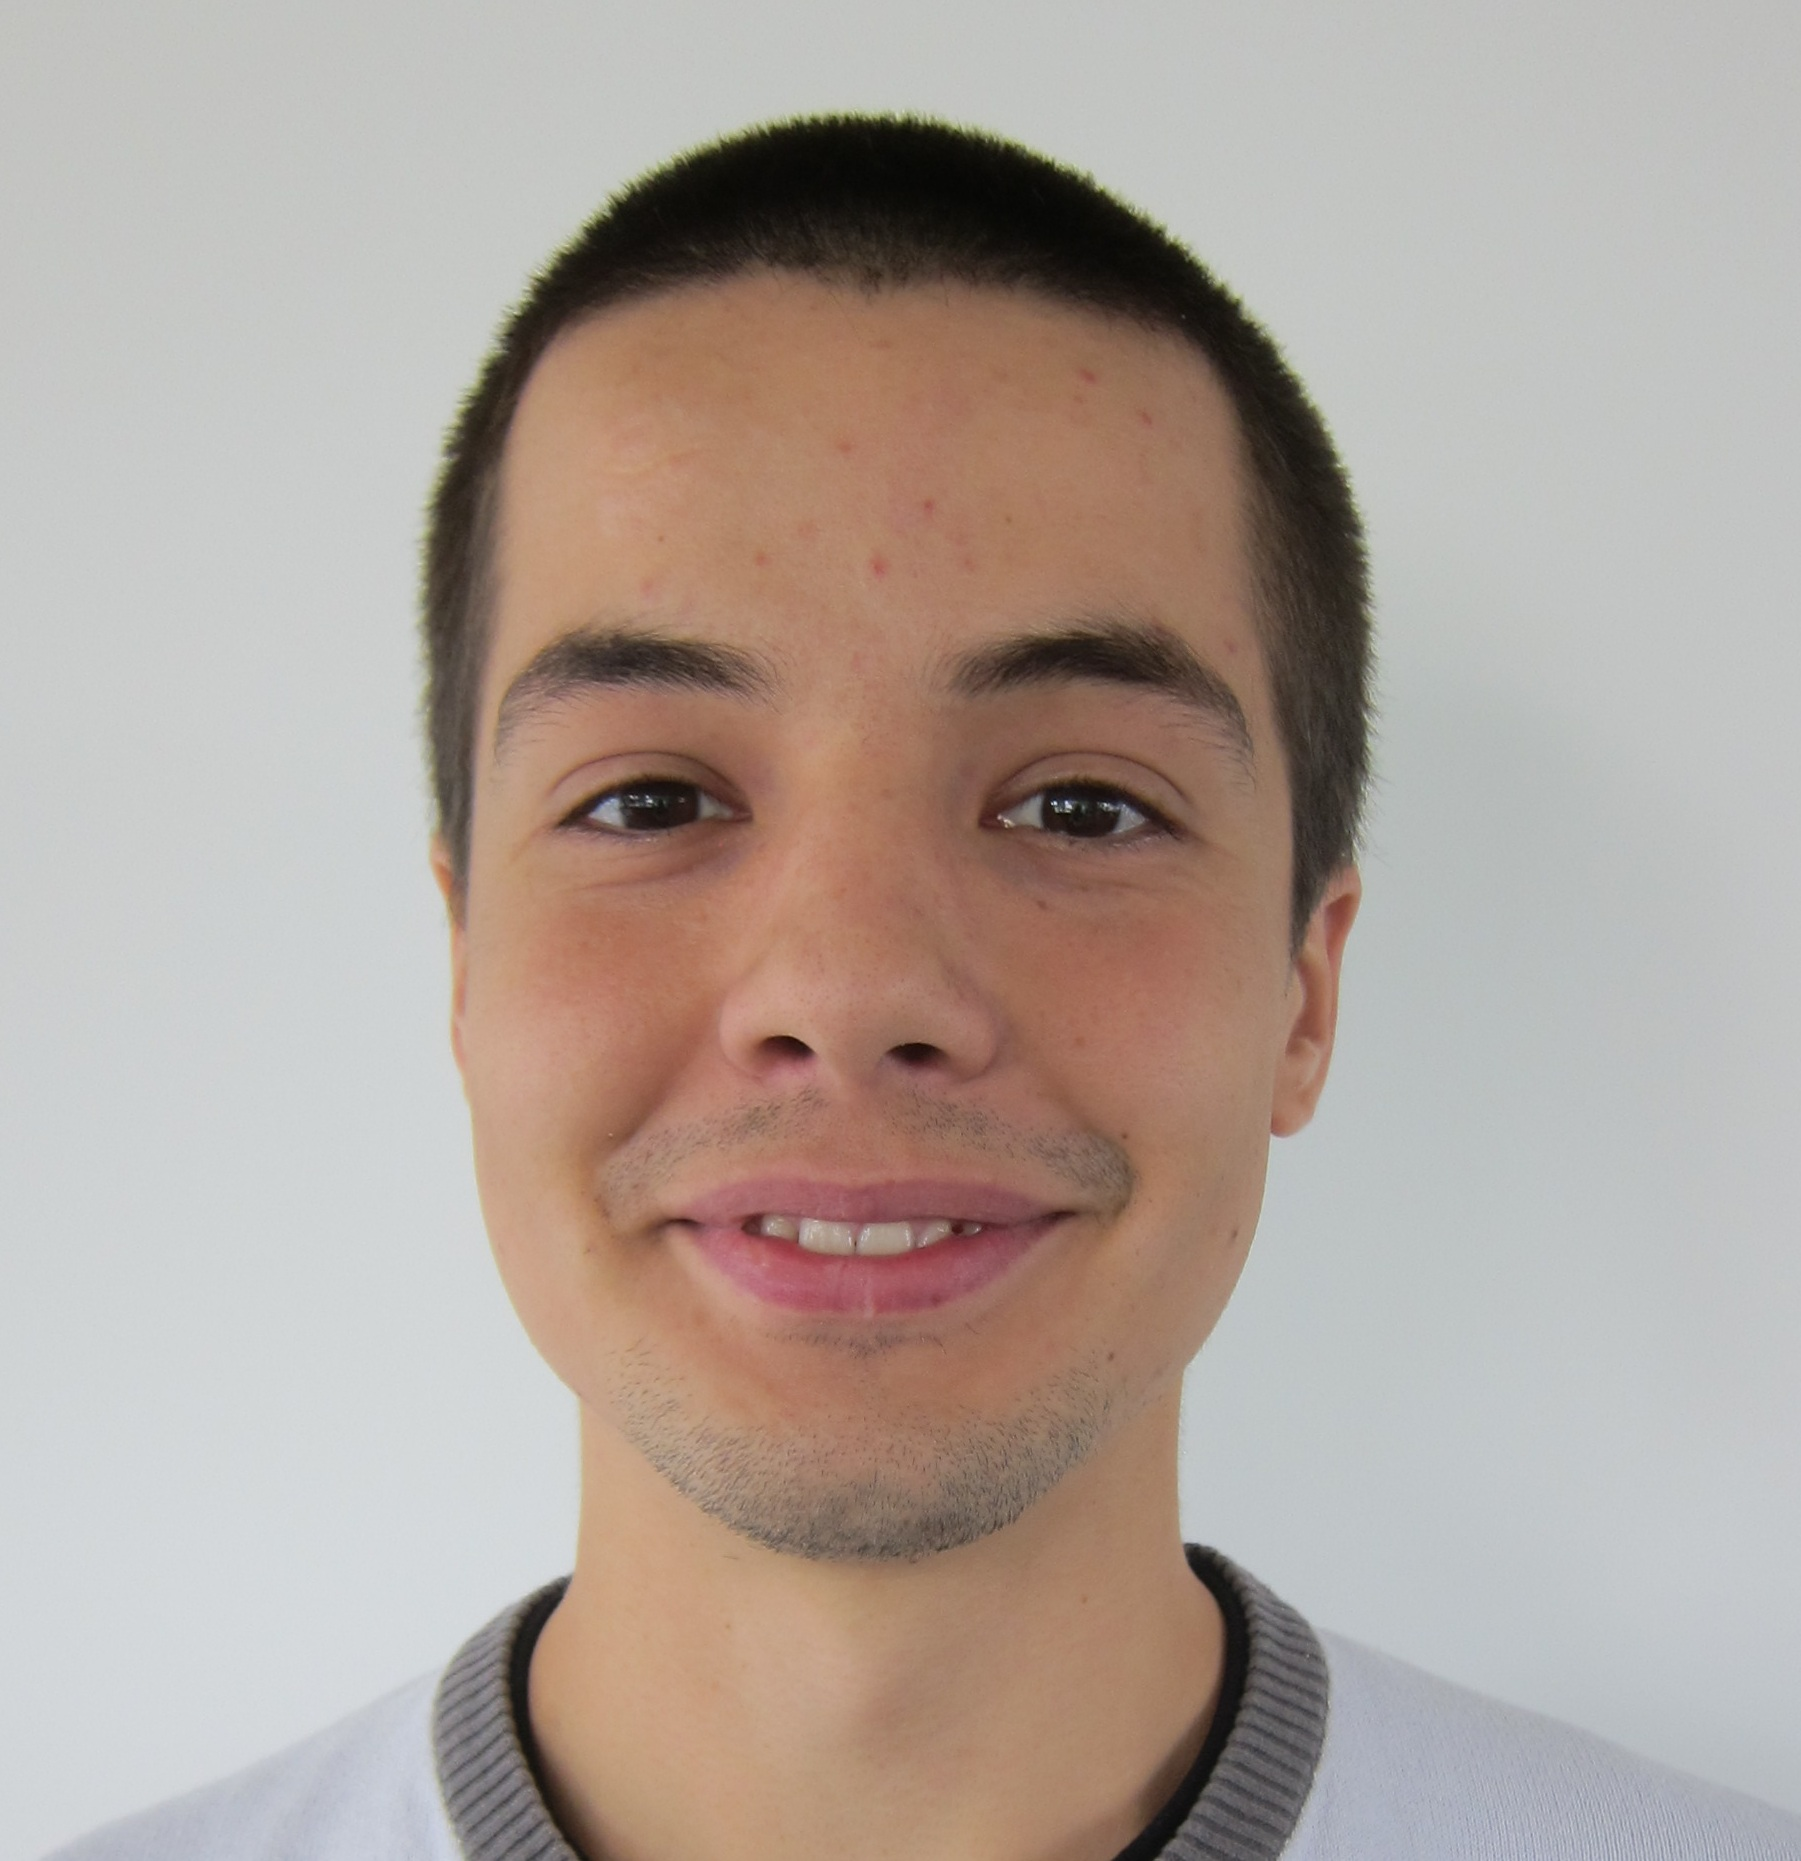
\includegraphics[width=3.4cm]{IMG_9061cropped3}%IMG_9061cropped3
        % bgMasterPhotoSmall
%         \includegraphics[width=3.7cm]
        % PersonalFotoBgMaster
      }%
     }%
  }%
}

%ptm phv pcr 
% \renewcommand{\rmdefault}{iwona}
% \renewcommand{\sfdefault}{iwona}
\usepackage[nodayofweek]{datetime}
\title{\bfseries\huge Iliya Stefanov Enchev\\
\addphoto{10}{138}}
\author{iliyastefanov@gmail.com}
\date{\today}
% \addphoto{5}{150}

\definecolor{lightgray}{gray}{0.8} 
\newcolumntype{L}{>{\raggedleft}p{0.17\textwidth}}
\newcolumntype{R}{p{0.8\textwidth}}
\newcommand\VRule{\color{lightgray}\vrule width 0.5pt}


% \begin{filecontents}{publication.bib}
% @article{lamport1986latex,
%   title={LaTEX: User's Guide \&amp; Reference Manual},
%   author={Lamport, L.},
%   year={1986},
%   publisher={Addison-Wesley}
% }
% @book{knuth2006art,
%   title={The art of computer programming: Generating all trees: history of combinatorial generation},
%   author={Knuth, D.E.},
%   volume={4},
%   year={2006},
%   publisher={addison-Wesley}
% }
% \end{filecontents} 

\begin{document}
% \addphoto{5}{150}


% 
\includegraphics{picture.jpg}
% \normalfont
% \maketitle
% \vspace{0.5em}
\section*{}
 
\begin{minipage}[ht]{0.68\textwidth} 
{\bfseries\huge Iliya Stefanov Enchev}\\
\newline
%iliyastefanov@gmail.com\\
iliyastefanov@gmail.com\\
+41 77 43 777 03\\
Rue Aloys-Mooser 3\\
1700 Fribourg\\
Switzerland\\
%Nationality: Bulgarian\\
% \formatdate{}{}{1986} 
Born: 29.03.1986
\end{minipage}
\begin{minipage}[ht]{0.48\textwidth}
% Nonlandian\\
% January 3rd, 2020\\
% +12 34 56 789

\addphoto{-111}{57}
% ~
% ~
% ~
% \newline
% \vspace{-15mm}
\vspace{112pt}  
\hspace{19mm} \longdate{\today}
\end{minipage}
\vspace{1pt}
%15pt


\section*{Objective}
I am applying for the position of LDBC Community manager. The LDBC project is
of particular interest to me, since I have worked on creating an RDF
benchmark \cite{bowlognaBench} and I have done evaluations with several other
benchmarks \cite{nosqlrdf}. I have experienced the need for more unified
standards in the field of RDF and Graph databases, where most solutions are
very specific and datasets vary widely in their structure so a
cross comparison is difficult. Realizing the seriousness of the issue
I'd be happy to help others in the field and spread the word of a
possible solution.
% After finishing my Master studies I took up the opportunity to
% work for a little while in the academic world, focusing on the Semantic Web and
% Linked Data. Now I am looking for a challenging long-term assignment, where I
% can pursue my interests in Software Engineering, Linked Data and Distributed
% Database Systems,
% %  and Systems Development,
% % Linked Data and Distributed
% % Systems, %and Systems Development
% and contribute with my practical knowledge,
% theoretical and analytical skills, and diverse international experience. For
% this reason I am applying as a Junior BIG DATA Engineer at ncx, Lausanne.

%acquired during my time at university and as a software engineer. 
% For this reason I am applying as a Junior/Professional Application Engineer at
% SBB, Bern.
% In the same time I hope to further develop my
%After finishing my Master's studies at Uni Fribourg in October '12 I took up
% the opportunity to work for a little while in Ireland and Fribourg in the academic
% field, focusing on Semantic Web and Linked Data. Now I am looking for a
% long-term assignment, where I can contribute with my theorethical and analytical skills, my practical
% knowledge and diverse international experience and in the same time pursue my
% interest in 
% Software Engineering and Data Management.
% further develop my interests in Software Engineering and Data handling
% Data. Now I would like to take advantage of my theorethical and analytical
% skills, my practical knowledge and diverse international experience.\\
%I finished my Master's studies .
%Having diverse international experience in the field of software engineering
% and more recently Linked Data and Semantic Web both in the industry and academic worldI am looking for an opportunity to apply d dsfdswdefwedf sdfsdfsfds fsfdssfsdfs fsdfsdfsdfsdf sdfsdfsdf fsdfsdfs fsd
%Find a job as a spaceship commander!

\section*{Relevant work experience}

\begin{tabular}{L!{\VRule}R}
Dec. 13--present&{\bf Research Associate at Ontotext}\\
&Collaboration on NoSQL data bases used as RDF stores.\\
Oct. 13--present&{\bf Software Engineer at ELCA}, Bern\\
&{\it ASTRA Verkehrs Management} -- Road traffic management project for the
Federal Roads Office. Responsabilities: developing new functionalities and bug
fixing.
Technologies: Java, GWTP, GXT, Hibernate, Spring, Maven etc.\\
Feb. 13--May 13&{\bf Scientific Collaborator at eXascale Infolab}, led by
Prof. Philippe Cudr\'e-Mauroux, University of Fribourg, Switzerland\\
&{\it NoSQL RDF Benchmark} -- Implementation of SPARQL with Apache
Jena on top of Couchbase document database for running Berlin and
DBpedia SPARQL Benchmarks on clusters of up to 16 nodes with large
datasets.\cite{nosqlrdf} \\
Jan. 11--May 12&{\it Project Bowlogna} -- Transforming relational
university data into RDF ontology and developing a Web visualization for
interaction with it. Developing ontology generator based on the same data.
Technologies: Jena, AllegroGraph, SPARQL, JavaScript, Ajax, jQuery, Cytoscape
Web.\cite{ bowlognaBench, bowlFost}\\

%\end{tabular}
%\begin{tabular}{L!{\VRule}R}
Nov. 12--Feb. 13&{\bf Collaborator at DERI}, Galway, Ireland, supervised by
Michael Hausenblas\\
&{\it Project Spitfire, LD4Sensors} -- Application for enriching sensor
metadata and sensor observations with Linked Data. Decoupling the
underlying RDF data store from the LD annotations layer, so that
data can be modified by other applications, updating the
REST API provided by the application.\\

%\end{tabular}

%\begin{tabular}{L!{\VRule}R}
% Jan. 11--May. 12&{\bf Collaborator at University of Fribourg}, Switzerland \\
% &{\it Project Bowlogna}--an application for generating ontologies of
% customizable size, based on real data from the Faculty of
% Humanities. Transforming relational university data into RDF ontology and
% developing a Web visualisation for interaction with it, using Jena,
% AllegroGraph, SPARQL, JavaScript, Ajax, jQuery, Cytoscape
% Web.\cite{ bowlognaBench, bowlFost}\\

%\end{tabular}

%\clearpage
%\section*{}
%\begin{tabular}{L!{\VRule}R}
Feb. 09--Aug. 10&{\bf Junior Software Engineer at Musala Soft}, Sofia, Bulgaria
\\
projects&{\it Barracuda for Mtel} -- %The biggest mobile operator in Bulgaria,
% part of Mobilkom Austria Group. 
Integration project for substituting legacy
billing%, ordering 
and CRM systems.\\
%  with products developed by Amdocs.\\
&{\it Declaration Management System (DMS)} with IBM Netherlands -- 
control and administation of movements
of goods through Dutch Customs.\\
&{\it Content Delivery Platform} for Mobilkom Austria, 
application for mobile entertainment content, % on mobile phones 
% -- games, ring tones, pictures 
accessible through Web or WAP interface.\\
responsibilities&Refactoring and testing PL/SQL procedures that extract
information relevant to billing cycles and different kinds of services and 
subscribers and provide this information to SAP 
accounting system. Code design, implementation and refactoring. 
%integration activities, close communication with team members, troubleshooting
%critical production issues. 
Technologies: Java EE, JSF, EJB, Hibernate ORM, Oracle DB.\\
\end{tabular}

\section*{IT Skills}
\begin{tabular}{L!{\VRule}R}
software development&Java SE/EE, JSP, JSF, Servlets,
Hibernate, JavaScript, JSON, Ajax, jQuery, Web Services, Oracle DB, SQL, PL/SQL, Apache
Cassandra, Couchbase, MapReduce, RDF, Apache Jena, SPARQL, Linux, Git, SVN
\\
% \end{tabular}
% 
% \section*{}
% \begin{tabular}{L!{\VRule}R}
% tools&dsdad\\
certification&Sun Certified Programmer for the Java Platform, Standard Edition 6\\
&Sun Certified Business Component Developer for the Java EE 5\\
\end{tabular}

% \section*{Master's thesis}
% \begin{tabular}{L!{\VRule}R}
% title&{\bf Unconventional Store Systems for RDF Data} \\
% supervisor&Prof. Philippe Cudr�-Mauroux\\
% description&Overview of some main points of the Web, Semantic Web and Linked Data. Presenting a number of registry
% systems that handle data broadly generalized as entities with identifiers -- DNS, DOA, ENS, Chord DHT and CoralCDN. 
% Comparison of four data storage solutions -- AllegroGraph, Open Chord, Apache
% Cassandra, MySQL in their ability to handle RDF entities, using a benchmarking
% suite developed in Java.\cite{downScale}
% \end{tabular}

\section*{Education}
\begin{tabular}{L!{\VRule}R}

%Presenting a number of registry systems that handle data broadly generalized
%as entities with identifiers -- DNS, DOA, ENS, Chord DHT and CoralCDN.
%Comparison of four data store solutions -- AllegroGraph, Open Chord, Apache
%Cassandra, MySQL in their ability to handle RDF entities, using a benchmarking
%suite developed in Java.\cite{downScale}\\
Sep. 10--Oct. 12&{\bf MSc in Computer Science,} Swiss Joint Master of
Science in Computer Science, Universities of Fribourg, Bern and Neuch\^atel,
Switzerland\\ %\vspace{5pt}
emphasis&Software Engineering -- several courses and three
projects based on GWT, Google maps API, SOAP, REST, MongoDB, Django; Agile
Methodologies; Data Management, Ubiquitous computing; Distributed Systems;
Concurrent programming.\\
Master's thesis&{\bf Unconventional Store Systems for RDF Data}\\
description&Overview on main points of the Web, Semantic Web and Linked
Data. Analysis and performance comparison of data store and entity registry
systems -- DNS, DOA, ENS, Chord DHT, CoralCDN, AllegroGraph, Apache
Cassandra and MySQL in their ability to handle RDF entities,
using own Java benchmarking suite.\cite{downScale}\\
2005--2009&{\bf BSc in Computer Science,} German Engineering Faculty of the
Technical University of Sofia, Bulgaria; courses taught in German\\
Mar. 08--Aug. 08&{\bf Erasmus exchange student,} Karlsruhe Institute of
Technology -- KIT, Germany
\end{tabular}







% \section*{Relevant work experience}
% \begin{tabular}{L!{\VRule}R}
% Jan. 11--May. 12&{\bf Collaborator at University of Fribourg}, Switzerland \\
% &{\it BowlognaBench}, an application that generates different sized ontologies based on real data from the university. Transforming relational data from the 
% Faculty of Humanities into RDF ontology and developing a Web visualisation for interaction with it, using Hibernate, 
% Jena, AllegroGraph, SPARQL, JavaScript, Ajax, jQuery, Cytoscape Web.\\  
% Feb. 09--Aug. 10&{\bf Junior Software Engineer,} Musala Soft, Sofia, Bulgaria \\
% Apr. 10--Aug. 10&{\it Project:} Barracuda for Mtel -- the biggest mobile operator in Bulgaria, part of Mobilkom
% Austria Group. Integration project for substituting legacy
% billing, ordering and CRM systems with products developed by Amdocs.\\
% &{\it Responsibilities:} Refactoring and testing PL/SQL procedures that extract
% information relevant to billing cycles and different kinds of services and 
% subscribers and provide this information to SAP 
% accounting system.\\
% Jun. 09--Mar. 10&{\it Project:} Declaration Management System (DMS) for Netherlands, designed to control movements
% of goods that go through Dutch Customs and are placed under Dutch Customs regulations.\\
% &{\it Responsibilities:} Code design and refactoring, implementation of new functionalities, according to 
% design specifications; integration and FAT activities, close communication with team members. Main tools used: JSF, EJB.\\
% Feb. 09--May. 10&{\it Project:} Content Delivery Platform for Mobilkom Austria Group, 
% an application that provides entertainment content for mobile phones -- games, ring 
% tones, pictures through Web or WAP interface.\\
% &{\it Responsibilities:} Code design, implementation and refactoring; 
% troubleshooting critical production issues, using mainly Java EE, Hibernate ORM, Oracle DB.\\
% \end{tabular}



\section*{Languages}
\begin{tabular}{L!{\VRule}R} 
Bulgarian&Mother tongue\\
English&Excellent C1 -- Certificate in Advanced English -- CAE; working in the
USA and Ireland\\
German&Excellent C1 -- DSH-Deutsche Sprachpr\"ufung f\"ur den Hochschulzugang\\
French&Intermediate B1 -- evening courses and courses at university, experience
in CH\\
Russian&Basic A2 -- second foreign language at secondary school
\end{tabular} 
 
\section*{Miscellaneous}
\begin{tabular}{L!{\VRule}R}
leisure&Cycling; swimming; playing a %Bulgarian 
folk
instrument -- gadulka; travelling; cooking;\\
%all sorts of bikes;
%swimming; 
%playing a Bulgarian folk instrument -- gadulka; travelling locally and %since
% elementary school
%abroad; cooking \\
soft skills&social networks, online hangouts for open source projects; a good
team player\\
driving license&A+B since 2004\\
\end{tabular}

    %\renewcommand\bibsection{\subsection{\refname}}
    
\renewcommand{\refname}{Publications}
\begingroup
    \fontsize{9pt}{11pt}\selectfont
\bibliographystyle{abbrv}%alpha plain abbrv
% \nobibliography{publication}

\bibliography{publication}
   %\renewcommand\@biblabel[1]{\textbullet}
% \nocite{*}
\endgroup
% \section*{Publications} 
\fontsize{14pt}{0pt}
%\selectfont
% \resizebox{\textwidth}{!}{
% \begin{tabular}{L!{\VRule}R} 
%\bibentry{downScale}
%\newline
%\bibentry{bowlFost} %\vspace{5pt} 
%\newline
%\bibentry{bowlognaBench}
% \end{tabular} 
%{%\vspace{20pt}\newline
% \vspace{5pt}
% \newline
% \newline
% \newline
% \vspace{5pt}
% \newline
%\vspace{35pt}
%\scriptsize\hfill Iliya Enchev \longdate{\today}} 
\end{document}